There are many factors that can cause problems in SAR images. An overview is presented in figure \ref{fig:overview}.
\begin{figure}[H]
    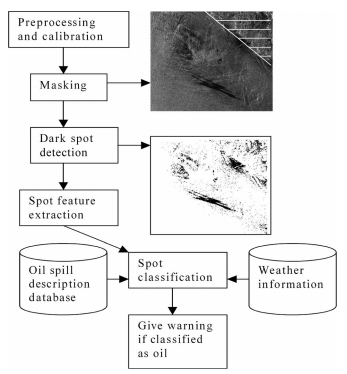
\includegraphics[width=80mm]{./img/detection_diagram.png}
    \caption{Overview for the oil spill detection approach \cite{Solberg200745}}
    \label{fig:overview}
\end{figure}
Preprocessing the SAR image is done to improve the contrast between dark spots and the water surrounding them, as well as flag certain dark spots to be ignored. 

First, there is a general quality assessment. If the image is blurred in general, it will be impossible to get any information out of it. Afterwards, experts look at noise removal. One of the most common versions of noise is speckle noise. Speckle noise is caused naturally by a disruption in the phase of radio waves. Radio waves leave the sensor all in the same phase. Once they interact with an object, they scatter and are out of phase with each other. If they interact with each other, the result will be a darker or lighter pixel than it should. Multi-look processing and spatial filtering can be done to reduce speckle noise \cite{simard1998analysis}.

Experts also flag (mask) areas in the image which might interfere with the classification process. These areas include shorelines, land and ships, as these would all be represented by dark areas in the images.
Another possibility is that dark spots are caused by algae or seaweed infestations \cite{fingas2014review}. Grease ice, rain cells and passing unknown vessels can all be mistaken for oil spills \cite{Brekke200595} so they need to be filtered out. 

These preprocessing steps will make classification easier, but is still a difficult task. In some cases a human expert can't even tell the difference \cite{Keramitsoglou2006640}. Through image segmentation, all dark spots are taken in isolation and the values of predefined features are extracted from them. Classification can now be performed by using the features as input where the output of the chosen classifier will be the probability of the dark spot being an oil spill or a lookalike. %THIS PART NEEDS A REFERENCE 
High or low wind areas are also taken into consideration as they change the surface of the water and oil slicks. This in turn could have influenced the reflection of radio waves and in turn the image \cite{fingas2014review}.

In an automated detection system, a high oil spill probability can lead to a warning message.


